\documentclass[12pt, twoside, openright]{report} % Fuente a 12pt, formato doble página y chapter a la derecha
\raggedbottom % No ajustar el contenido con un salto de página

% MÁRGENES: 2,5 cm sup. e inf.; 3 cm izdo. y dcho.
\usepackage[
a4paper,
vmargin=2.5cm,
hmargin=3cm
]{geometry}

% INTERLINEADO: Estrecho (6 ptos./interlineado 1,15) o Moderado (6 ptos./interlineado 1,5)
\renewcommand{\baselinestretch}{1.15}
\parskip=6pt

% DEFINICIÓN DE COLORES para portada y listados de código
\usepackage[table]{xcolor}
\definecolor{azulUC3M}{RGB}{0,0,102}
\definecolor{gray97}{gray}{.97}
\definecolor{gray75}{gray}{.75}
\definecolor{gray45}{gray}{.45}

% Soporte para GENERAR PDF/A
\usepackage{etoolbox}
\makeatletter
\@ifl@t@r\fmtversion{2021-06-01}%
 {\AddToHook{package/after/xmpincl}
   {\patchcmd\mcs@xmpincl@patchFile{\if\par}{\ifx\par}{}{\fail}}}{}
\makeatother
\usepackage[a-1b]{pdfx}

% ENLACES
\usepackage{hyperref}
\hypersetup{colorlinks=true,
  linkcolor=black, % enlaces a partes del documento (p.e. índice) en color negro
  urlcolor=blue} % enlaces a recursos fuera del documento en azul

% Añadir pdfs como partes del documento
\usepackage{pdfpages}

% Quitar la indentación de principio de los párrafos
\setlength{\parindent}{0em}

% EXPRESIONES MATEMÁTICAS
\usepackage{amsmath,amssymb,amsfonts,amsthm}

\usepackage{txfonts} 
\usepackage[T1]{fontenc}
\usepackage[utf8]{inputenc}

% Insertar gráficas y fotos
\usepackage{tikz}
\usepackage{pgfplots}

\usepackage[spanish, es-tabla]{babel} 
\usepackage[babel, spanish=spanish]{csquotes}
\AtBeginEnvironment{quote}{\small}

% diseño de PIE DE PÁGINA
\usepackage{fancyhdr}
\pagestyle{fancy}
\fancyhf{}
\renewcommand{\headrulewidth}{0pt}
\fancyfoot[LE,RO]{\thepage}
\fancypagestyle{plain}{\pagestyle{fancy}}

% DISEÑO DE LOS TÍTULOS de las partes del trabajo (capítulos y epígrafes o subcapítulos)
\usepackage{titlesec}
\usepackage{titletoc}
\titleformat{\chapter}[block]
{\large\bfseries\filcenter}
{\thechapter.}
{5pt}
{\MakeUppercase}
{}
\titlespacing{\chapter}{0pt}{0pt}{*3}
\titlecontents{chapter}
[0pt]                                               
{}
{\contentsmargin{0pt}\thecontentslabel.\enspace\uppercase}
{\contentsmargin{0pt}\uppercase}                        
{\titlerule*[.7pc]{.}\contentspage}                 

\titleformat{\section}
{\bfseries}
{\thesection.}
{5pt}
{}
\titlecontents{section}
[5pt]                                               
{}
{\contentsmargin{0pt}\thecontentslabel.\enspace}
{\contentsmargin{0pt}}
{\titlerule*[.7pc]{.}\contentspage}

\titleformat{\subsection}
{\normalsize\bfseries}
{\thesubsection.}
{5pt}
{}
\titlecontents{subsection}
[10pt]                                               
{}
{\contentsmargin{0pt}                          
  \thecontentslabel.\enspace}
{\contentsmargin{0pt}}                        
{\titlerule*[.7pc]{.}\contentspage}  

% DISEÑO DE TABLAS.
\usepackage{multirow} % permite combinar celdas 
\usepackage{caption} % para personalizar el título de tablas y figuras
\usepackage{floatrow} % utilizamos este paquete y sus macros \ttabbox y \ffigbox para alinear los nombres de tablas y figuras de acuerdo con el estilo definido. Para su uso ver archivo de ejemplo 
\usepackage{array} % con este paquete podemos definir en la siguiente línea un nuevo tipo de columna para tablas: ancho personalizado y contenido centrado
\newcolumntype{P}[1]{>{\centering\arraybackslash}p{#1}}
\DeclareCaptionFormat{upper}{#1#2\uppercase{#3}\par}

% Diseño de tabla para ingeniería
\captionsetup[table]{
  format=hang,
  name=Tabla,
  justification=centering,
  labelsep=colon,
  width=.75\linewidth,
  labelfont=small,
  font=small,
}

% DISEÑO DE FIGURAS.
\usepackage{graphicx}
\graphicspath{{img/}} %ruta a la carpeta de imágenes

% Diseño de figuras para ingeniería
\captionsetup[figure]{
  format=hang,
  name=Fig.,
  singlelinecheck=off,
  labelsep=colon,
  labelfont=small,
  font=small    
}

% NOTAS A PIE DE PÁGINA
\usepackage{chngcntr} % Para numeración continua de las notas al pie
\counterwithout{footnote}{chapter}

% LISTADOS DE CÓDIGO
% soporte y estilo para listados de código. Más información en https://es.wikibooks.org/wiki/Manual_de_LaTeX/Listados_de_código/Listados_con_listings
\usepackage{listings}

% definimos un estilo de listings
\lstdefinestyle{estilo}{ frame=Ltb,
  framerule=0pt,
  aboveskip=0.5cm,
  framextopmargin=3pt,
  framexbottommargin=3pt,
  framexleftmargin=0.4cm,
  framesep=0pt,
  rulesep=.4pt,
  backgroundcolor=\color{gray97},
  rulesepcolor=\color{black},
  %
  basicstyle=\ttfamily\footnotesize,
  keywordstyle=\bfseries,
  stringstyle=\ttfamily,
  showstringspaces = false,
  commentstyle=\color{gray45},     
  %
  numbers=left,
  numbersep=15pt,
  numberstyle=\tiny,
  numberfirstline = false,
  breaklines=true,
  xleftmargin=\parindent
}

\captionsetup[lstlisting]{font=small, labelsep=period}
% fijamos el estilo a utilizar 
\lstset{style=estilo}
\renewcommand{\lstlistingname}{\uppercase{Código}}

\pgfplotsset{compat=1.17} 
%-------------
% DOCUMENTO
%-------------

\begin{document}
\pagenumbering{roman} % Se utilizan cifras romanas en la numeración de las páginas previas al cuerpo del trabajo

%----------
% PORTADA
%---------- 
\begin{titlepage}
	\begin{sffamily}
		\color{azulUC3M}
		\begin{center}
			\begin{figure}[H] %incluimos el logotipo de la Universidad
				\makebox[\textwidth][c]{
\includegraphics[width=16cm]{Portada_Logo.png}}
			\end{figure}
			\vspace{2.5cm}
			\begin{Large}
				Grado en Ingeniería Informática\\
				2021-2022\\
				\vspace{2cm}
				\textsl{Apuntes}\\
				\bigskip
			\end{Large}
			{\Huge Redes de Neuronas Artificiales}\\
			\vspace*{0.5cm}
			\rule{10.5cm}{0.1mm}\\
			\vspace*{0.9cm}
			{\LARGE Jorge Rodríguez Fraile\footnote{\href{mailto:100405951@alumnos.uc3m.es}{Universidad: 100405951@alumnos.uc3m.es}  |  \href{mailto:jrf1616@gmail.com}{Personal: jrf1616@gmail.com}}}\\
			\vspace*{1cm}
		\end{center}
		\vfill
		\color{black}
		
\includegraphics[width=4.2cm]{img/creativecommons.png}\\
		Esta obra se encuentra sujeta a la licencia Creative Commons\\ \textbf{Reconocimiento - No Comercial - Sin Obra Derivada}
	\end{sffamily}
\end{titlepage}

%----------
% ÍNDICES
%---------- 

%--
% Índice general
%-
\tableofcontents
\thispagestyle{fancy}

%--
% Índice de figuras. Si no se incluyen, comenta las líneas siguientes
%-
\listoffigures
\thispagestyle{fancy}

%--
% Índice de tablas. Si no se incluyen, comenta las líneas siguientes
%-
\listoftables
\thispagestyle{fancy}

%----------
% TRABAJO
%---------- 

\pagenumbering{arabic} % numeración con múmeros arábigos para el resto de la publicación  


%----------
% COMENZAR A ESCRIBIR AQUI
%---------- 

\chapter{Información}

\section{Profesores}
\begin{quote}
	Magistral: Isasi Viñuela, isasi@ia.uc3m.es
	
	Prácticas: José María Valls, jvalls@inf.uc3m.es
	
	Inés M. Galván, igalvan@inf.uc3m.es (de baja)
\end{quote}

\section{Objetivos}
\begin{itemize}
	\item “Transmitirnos su entusiasmo por las redes neuronales”, darnos la posibilidad de acceder más fácilmente a este mundo.
	\item Entender que subyace sobre estas redes y el método científico.
	\item Estudiar los diferentes modelos de redes.
	\item Describir las diferentes áreas de aplicabilidad de las redes de neuronas.
	\item Resolver problemas con redes de neuronas.
	\item Analizar las ventajas e inconvenientes de neuronas.
	\item Analizar las ventajas e inconvenientes de cada uno de los modelos de redes desde una perspectiva aplicada.
	\item Diseñar un conjunto de experimentos para la resolución de problemas.
\end{itemize}

\section{Sistema de evaluación}
\begin{itemize}
	\item 60 \% Evaluación continua
	      \begin{itemize}
		      \item 20 \% Practica 1. Trata de resolver un problema de regresión, estimar un número real, y se divide en dos partes:
		            \begin{itemize}
			            \item  Modelo lineal (ADALINE) determinando los coeficientes, este caso tenemos programarlo nosotros en nuestro lenguaje de preferencia.
			                  Se nos proporcionan unos datos de prueba para cuando lo estemos programando salga un error muy pequeño, de esta manera sabemos si lo hacemos bien. Las de prueba son 3 atributos, pero los reales son de 8.
			            \item  No lineal (Perceptrón multicapa), presentando una memoria de unas 8 páginas en forma de artículo.
			                  Para esta parte se nos dará un script en R, no hay que programarlo, pero hay que realizar muchas pruebas para ver los resultados (errores).
		            \end{itemize}
		      \item 20 \% Practica 2. Habrá que modificar scripts de Python, también se usará Google Colab.
		            \begin{itemize}
			            \item Parte 1: Problema de clasificación que resolveremos con Perceptrón multicapa.
			            \item Parte 2: Problema de clasificación con imágenes usando Deep Learning.
		            \end{itemize}
		      \item 20 \% Prueba parcial, de las prácticas (a principios de noviembre).
	      \end{itemize}
	\item 40 \% Examen final, se realizarán cuestiones teórico-prácticas, pudiendo incluir preguntas sobre las prácticas.
	      \begin{itemize}
		      \item Se puede emplear material.
		      \item No hay nota mínima
	      \end{itemize}
\end{itemize}

Para la bibliografía se empleará en los primeros temas el libro escrito por los profesores (Redes de Neuronas Artificiales. Un enfoque práctico, 2004), pero para el resto de los temas sobre todo Deep Learning (Redes Neuronales \& Deep Learning de Fernando Bernal, 2018).

\chapter{Practica 1}
\section{Preparación de Datos}
\subsection{Los datos}
Variables, datos o patrones de entrada y de salida deseada de la red, que solo trabajan con atributos numéricos y cuando no son numéricos se discretizan para que pasen a ser numéricos.

\textbf{Supervisado:} Hay una salida que es lo que buscamos determinar.

\textbf{No supervisado:} Tratamos de agrupar o buscar una determinada estructura en los datos, no hay salida.

\subsection{Transformación de los datos}
\textbf{Normalización de datos:} Se emplea en los casos en los que los valores entre los atributos con muy dispares (ej. 0.1 y 10) lo que provocaría que al realizar operaciones entre ellos dieran valores que dependen mucho más de un atributo que otro. Los valores se ajustan al rango de 0 y 1.

$$ValorNormalizado_i=\frac {Valor_i-ValorMinimo_i} {ValorMaximo_i-ValorMinimo_i}$$

\textbf{Aleatorización de los datos:} Se altera el orden las instancias de manera que se evita cualquier sesgo a la hora de entrenar el modelo.

\textbf{Eliminación de  atributos irrelevantes:} Nosotros no lo haremos, pero este nos permite eliminar la información que no aporta nada y entorpece el entrenamiento.

\textbf{Reducción dimensionalidad:} Se realizan las técnicas de reducción de dimensionalidad, que bien seleccionan un subconjunto de atributos, bien transforman los datos de entrada en otro conjunto de mayor dimensión.

\subsection{Evaluación de una red de Neuronas}
\textbf{Separación del conjunto de entrenamiento y test:} Se separa un conjunto de instancias que se emplearan solo para el entrenamiento y otro que se utilizara solo para evaluar el modelo, el conjunto de test. Esto permitirá detectar si el entrenamiento que estamos haciendo se está sobreajustando, haciendo que no generalizase adecuadamente.
\pagebreak

\textbf{Validación cruzada:} Consiste en dividir los datos en una serie de conjuntos de igual tamaño. Con estos conjuntos se va entrenando, dejando uno fuera en todo momento para utilizarlo como test. Esto nos permite evaluar el error haciendo la media de todos los errores obtenidos con los modelos, siendo este valor error del modelo que se obtienen entrenando con todas las instancias.

\textbf{Validación cruzada estratificada:} Se dividen de igual las instancias en conjuntos de igual tamaño. En este caso lo que se hace es que haya en cada conjunto la misma proporción de instancias con cada clase con respecto al total. Todos tendrán la misma proporción de instancias de una clase que los otros del total.
Lo que se hace es separar las instancias por la clase, de estos conjuntos generados se divide cada uno en el número de conjuntos de validación cruzada, de esta manera en cada uno de los conjuntos que vamos a generar vamos cogiendo uno conjunto de cada una de las clases.

\textbf{Medida de evaluación}
\begin{itemize}
	\item \textbf{En regresión:} Error absoluto medio (Mean Absolute Error) es la media del valor absoluto de la diferencia de la salida y el deseado. Error cuadrático medio (Mean Square Error) es igual al anterior, pero en vez de valor absoluto la diferencia se pone al cuadrado.
	      $$MAE=\frac 1 N \sum^N_{i=1} |s_i-d_i| \quad MSE=\frac 1 N \sum^N_{i=1} (d_i-s_i)^2$$
	      Acaba cuando el error medio o el cuadrático es aceptable. También por una visualización gráfica de las salidas deseadas y las salidas de la red.
	\item \textbf{En clasificación:} Lo más habitual es evaluar la calidad de la red basándonos en su precisión predictiva (\% de aciertos), la proporción de aciertos sobre el total de instancias.
	      
	      Acaba cuando el porcentaje de aciertos es alto, teniendo en cuenta que debe ser mayor que la probabilidad de que acierte aleatoriamente (como si tirase una moneda) y las clases están equilibradas (porque si siempre da una clase podría tener un buen porcentaje de acierto dando un valor constante).
	      
	      \textbf{Matriz de confusión:} Representa la cantidad de instancias según lo estimado y lo correcto, de manera que se pueda ver los que han sido estimados según TP, FN, FP o TN. Los datos correctamente clasificados están en la diagonal, los incorrectos fuera de ella. Se emplean otras medidas como son:
	      \begin{itemize}
		      \item El porcentaje de aciertos total es $\frac {TP+TN} {TP+TN+FN+FP}$
		      \item El porcentaje de aciertos de + es: $\frac {TP} {TP+FN}$
		      \item El porcentaje de aciertos – es: $\frac {TN} {FP+TN}$
	      \end{itemize}
	      
\end{itemize}

\subsection{Anotaciones Practica 1}
A la hora de normalizar hacerlo sobre el total de los datos, no solo sobre los de entrenamiento.
Aleatorizarlos.
Separar las instancias en 70 15 15.

En la parte de programar los vectores de pesos y umbrales, si se hace un vector con los pesos y el umbral, tener en cuenta que al hacer el producto cartesiano el de entrada debe tener un 1 para el umbral. $[x_1 \; x_2 \; x_3 \; 1]$ con $[w_1 \; w_2 \; w_3 \; \sigma]$

\chapter{Tema 1: Introducción}
El objetivo de la IA es la construcción de sistemas inteligentes.

\textbf{Sistema Inteligente:} Dispositivo físico o lógico con capacidades propias de los humanos como tomar decisiones, resolución de problemas o el aprendizaje.

Partiremos de la base, por lo que el primer paso serán organismos más pequeños, pero el objetivo es alcanzar la capacidad humana y llegar a sustituirnos.

Áreas
\begin{itemize}
	\item \textbf{Simbólica (Top-down):} Diseñar componentes del sistema inteligente donde el comportamiento es programado por nosotros para que él sea capaz de razonar y aprender. Se emplea en búsqueda y optimización
	\item \textbf{Subsimbólica (Bottom-up):} Se programa lo básico y lo dejamos interactuar para ver si llega a un punto adecuado. No programamos el comportamiento, sino las partes base y miramos a ver como se relaciona y si lo resuelve.
\end{itemize}

Las \textbf{Redes de Neuronas} se encuentran en la IA subsimbólica, tratan de emular los sistemas neuronales biológicos. Se ha estado durante décadas detrás de la construcción de algoritmos capaces de procesar la información de la misma manera que lo hace el cerebro humano.

Se caracterizan por tener la \textbf{propiedad de aprender} a partir de ejemplos.

Tratan \textbf{información numérica}, si se puede discretizar bien, si no se emplean otros métodos.

En la actualidad existe un gran número de arquitecturas diferentes de redes de neuronas artificiales, además este progreso ha sido posible por la capacidad de cómputo, esos procesos son muy costosos.

Algunas \textbf{áreas de aplicación}:
\begin{itemize}
	\item Reconocimiento de patrones (imagen, voz, caracteres)
	\item Compresión y análisis de datos.
	\item Robótica.
	\item Medicina.
	\item Predicción de series temporales.
\end{itemize}

Las redes de neuronas no permiten abordar problemas de: Aproximación, Predicción, Clasificación, Agrupación.

\textbf{Otras técnicas de IA que se pueden emplear} para estos problemas son:
\begin{itemize}
	\item Máquinas de Vectores de Soporte (Vapnik, 1995)
	\item Gradient Boosting (Friedman, 2002)
	\item Random Forest (Breiman, 2001)
	\item K-medias (agrupación) (MacQueen, 1967)
\end{itemize}

\textbf{Ventajas}
\begin{itemize}
	\item Son fáciles de utilizar y diseñar, la parte difícil es acertar.
	\item Capacidad de aprender a partir de ejemplos.
	\item Tolerancia al ruido en los ejemplos, es muy tolerante a fallos, incluso a la perdida de unas pocas neuronas.
	\item Diversidad de las áreas de aplicación, teniendo datos se puede aplicar en problemas de cualquier área aunque no seamos expertos en la misma.
\end{itemize}

Desde la aparición de las redes sociales y móviles las compañías han recogido muchísimos datos que han posibilitado el entrenamiento de  redes en muchas áreas.

\textbf{Problemas específicos de las RNA}
\begin{itemize}
	\item Tiempo de aprendizaje, requiere mucha capacidad de cómputo y son lentos.
	\item Determinación de los hiperparametros, como el número de neuronas, ciclos, etc.
	\item No se pueden explicar los resultados, como una caja negra por lo que se están diseñando redes cuyo propósito es explicar.
\end{itemize}

\section{Historia}
Comienza en \textbf{1940} con estudios en la neurocirugía, al descubrir la neurona, se empezó a ver el funcionamiento del cerebro y se vio que funcionaba por señales eléctricas. A raíz de esto se hicieron modelos computaciones basados en lo que se conocía, se crearon para puertas lógicas inicialmente (con pesos fijos). El primer modelo fue de S. McCulloch y W. Pitts, que permitía pesos que se ajustaban, pero no se aprendían.

F. Rosenblatt en \textbf{1957} diseñó el Perceptrón que tenía un proceso para calcular los pesos según las entradas, en esos momentos la entrada era binaria.

B. Widrow y M. Hoff en \textbf{1960} diseñaron el \textbf{ADALINE} que permitía entradas no binarias.

Faltaban neuronas por falta de hardware, pero se pensaba que ya estaba todo hecho.

M. Minsky y S. Papert con el \textbf{libro “Perceptrón”} en \textbf{1969} rompieron el pensamiento de que todo estaba hecho con el \textbf{XOR Problem}, en el que no existe un único plano que represente la logia de la puerta XOR. Este problema inició la Época oscura (“AI Winter”).

D. Rumelhart, G. Hinton y R. William en \textbf{1986} solucionaron el problema XOR con más de 1 capa en el perceptrón, lo que da origen al \textbf{Perceptrón Multicapa y la Retropropagación.}

V. Vapnik y C. Cortes en \textbf{1995} desarrollaron las Máquinas de Vectores de Soporte (SVM) que están relacionados con problemas de clasificación y regresión.

En el año \textbf{2006} ya había capacidad de cómputo, se podía dar más profundidad con un mayor número de capas \textbf{Redes de Neuronas Profundas}, pero no se avanzó mucho en la teoría, se basaba en lo que había dicho Rumelhart.

\section{Fundamentos biológicos}
El \textbf{Sistema nervioso} es un conjunto de células especializadas en la conducción de señales eléctricas. Capta estímulos del entorno o internos, procesa la información y genera respuestas diferentes según la situación. No todos son igual de complejos, la estructura es lo que varía, pero todos están compuestos por los mismos componentes.

El \textbf{Cerebro} es el órgano principal del Sistema Nervioso. Se encarga de regular y mantener cada función vital del cuerpo, y es el órgano donde reside la mente y la conciencia del individuo. Existen distintas áreas, cada una más sofisticada para una serie de tareas (como puede ser la motora, sensoria, etc.), pero todas son importantes para el individuo.
\begin{itemize}
	\item Está formado por $10^{11}$ células, llamadas neuronas, interconectadas entre sí (cada una a otras 1000-10000 $10^{15}$) y forman una densa red.
\end{itemize}

Las neuronas se comunican a través de \textbf{impulsos eléctricos de corta duración, que se transmiten a través de las sinapsis}.

El impulso se propaga a través del axón, y es recibido por la dendrita (ramificaciones de la neurona que buscan axones) de la célula receptora.

El \textbf{Axón} (una sola por neurona) se ramifica, y puede propagar una misma señal a cientos de dendritas de células diferentes. Contiene unas vesículas que contienen los neurotransmisores, que al liberarse se comunican con la neurona inmediata por medio de la sinapsis. La señal que se propaga es única y es recibida por todas las células conectadas.

Las \textbf{Dendritas} reciben multitud de señales diferentes, algunas excitatorias y otras inhibitorias.
\pagebreak

Cuando el impulso llega a la neurona pre-sináptica, abre los canales de ion cálcico que liberan los neurotransmisores que son captados por los receptores de la neurona post-sináptica que abren o cierran los canales iónicos de la dendrita generando potenciales eléctricos que permiten la propagación de la señal hacia el soma de la célula. Se va despolarizando al recibir estímulos eléctricos, cuando supera un umbral se dispara un potencial de acción.

\textbf{Son elementos no lineales:} Si se supera un umbral, se produce una señal de activación

El sistema nervioso funciona como una enorme malla que propaga señales electroquímicas de unas células a otras, modificando sucesivamente la concentración de iones de las sinapsis.

Robustez y tolerancia a fallos

Adaptación y plasticidad

Manejar información: inconsistente, difusa y con ruido

Una \textbf{red artificial (ResNet152) puede llegar a los 60 millones de sinapsis} (diez millones de veces más pequeña), todavía estamos lejos.

\section{Neurona artificial}
Trata de imitar las características generales de las neuronas.
\begin{figure}[H]
	\ffigbox[\FBwidth]
	{\caption{Comparación neurona bilógica y neurona artificial}}
	{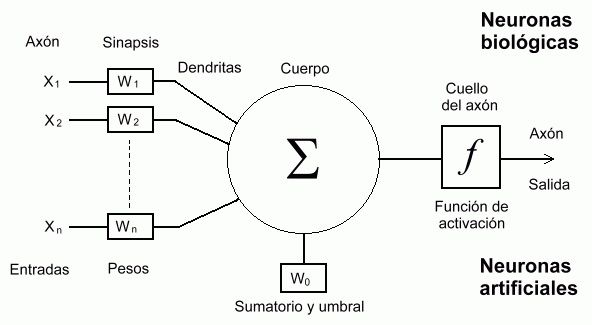
\includegraphics[scale=.8]{neurona-vs-perceptron.jpg}}
\end{figure}

Las \textbf{dendritas funcionan como las entradas} en la neurona, el \textbf{axón como la salida} y la \textbf{densidad de la sinapsis para que pase mejor el impulso serían los pesos}.

En cuanto al \textbf{potencial de acción (cuando supera el umbral) se simula con una función de activación} no lineal. Se utiliza un \textbf{umbral para poder ajustar esta función}.

Cada neurona está caracterizada por un estado interno denominado nivel de activación:
\begin{itemize}
	\item Discreto: Desactivado o Activado, S=0,1.
	\item Continuo: S=[0,1].
\end{itemize}

\textbf{Función de activación:} permite cambiar el nivel de activación a partir de las señales de entrada.

Las señales de entrada se combinan entre sí, generando la entrada total.

\textbf{Tipos de funciones de activación:}
\begin{figure}[H]
	\ffigbox[\FBwidth]
	{\caption{Tipos de funciones de activación}}
	{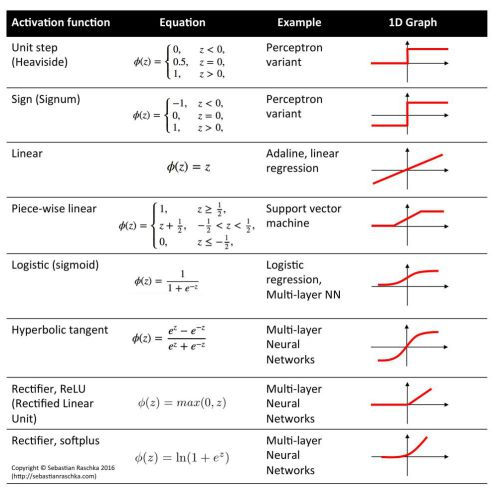
\includegraphics[scale=.8]{tipos-fun-act.jpg}}
\end{figure}

Las que nosotros emplearemos con la Sigmoide, Tangente hiperbólica y la ReLU (Rectified Linear Unit, es lineal a partir de 0).

Excepto la función lineal estas propagan la señal de manera no lineal.
\pagebreak

\subsection{Modelo computacional}
\textbf{Componentes}
\begin{itemize}
	\item Conjunto de unidades de proceso o neuronas artificiales.
	\item Conexiones entre las unidades.
	\item Regla de propagación, para propagar las entradas hacia la salida de la red.
	\item Regla de aprendizaje para modificar los pesos de las conexiones.
\end{itemize}

Tiene una arquitectura en forma de capas (entrada, ocultas y salida) que se propaga hacia delante (izq. a dch.).

Las capas ocultas son las que realizan el procesamiento, la entrada y salida solo se encargan de recibir y sacar los datos de la red.

Las conexiones van de una capa a la inmediata siguiente, no saltan capas o retroceden (todavía no). Todas las neuronas de una capa están conectadas con cada una de la capa anterior y posterior (full connected).

El aprendizaje consiste en ajustar los pesos de tal manera que pueda resolver el problema de manera eficaz.

\subsection{Aprendizaje}
Tratamos de que al pasar un patrón (serie de datos de entrada) nos dé la salida correspondiente, para esto cuando falla hay que ajustar los pesos y umbral.

Se realiza a partir de un conjunto de ejemplos o muestras conocidas, que llamaremos Conjunto de entrenamiento. Se debe disponer de una cantidad significativa y representativa de ejemplos para realizar un buen aprendizaje, suficientes ejemplos y que cubran la variedad de salidas.

\textbf{Proceso:}
\begin{enumerate}
	\item Introducir progresivamente los ejemplos de aprendizaje.
	\item Modificar los pesos siguiendo una ley o ecuación de aprendizaje.
	\item Cuando se han introducido todos se ha completado una iteración. Ahora se comprueba si se cumple cierto criterio de convergencia y si no se cumple, se repite el proceso.
\end{enumerate}
\pagebreak

La modificación de los pesos puede ocurrir después de introducir cada patrón (lo habitual) o después de introducir todos los patrones (o un lote de estos, permite acelerar el proceso y se usa en Redes Convolucionales).

En cuanto a la finalización del aprendizaje se hace en función de un criterio de convergencia que puede ser que el error sea menor que un valor dado (puede no llegar a ocurrir) o que los pesos dejen de sufrir modificaciones y el error se estabilice.

\textbf{Modelos de aprendizaje:}
\begin{itemize}
	\item \textbf{Aprendizaje supervisado:} Se conoce la salida de los ejemplos de aprendizaje. Utiliza un proceso externo para determinarlo. Conocer el resultado nos permite manejar el error cometido y guiar el aprendizaje
	\item \textbf{Aprendizaje no supervisado:} No se conoce la salida de los ejemplos. Permite detectar características de los datos, agruparlos o reducir la dimensionalidad. Se reajustan automáticamente los pesos y autoorganiza la información.
	\item \textbf{Aprendizaje por refuerzo:} Se aprende por prueba y error guiado por una recompensa si lo hace bien. No existe medida de error, solo si lo ha habido.
\end{itemize}

\subsection{Validación}
El modelo resultante debe ser capaz de responder de forma adecuada ante datos desconocidos. Meter datos no conocidos y usarlos solo para evaluar (no aprender) si el modelo es bueno.

El conjunto de datos disponibles se divide en subconjuntos de:
\begin{itemize}
	\item \textbf{Entrenamiento:} Usado para ajustar el valor de los pesos.
	\item \textbf{Validación (no siempre se utiliza este conjunto):} Usado para determinar los hiperparámetros de la red y detener el aprendizaje. Permite detectar sobre ajuste.
	\item \textbf{Test:} Usado para medir la capacidad de generalización de la red. Se utiliza este segundo no conocido porque no es conocido y no se ha utilizado previamente (ni entrenar, ni para el entrenamiento) son verdaderamente nuevos para el modelo.
\end{itemize}

Los conjuntos de validación y test deben ser Independientes del aprendizaje, Significativos y representativos.

\textbf{Sobreajuste (overfitting):} La red se ha sobreajustado a los ejemplos de entrenamiento, deja de generalizar bien.
\pagebreak

\subsection{Taxonomía}
Redes Feedforward supervisadas: Conexiones hacia delante y aprendizaje supervisado.
\begin{itemize}
	\item Perceptrón simple, Adaline, Perceptrón Multicapa, Redes de Base Radialy Redes Convolucionales.
\end{itemize}

Redes no supervisadas
\begin{itemize}
	\item Kohonen y ART.
\end{itemize}

Redes recurrentes: Conexiones en todas las direcciones
\begin{itemize}
	\item Solo unas pocas conexiones recurrentes: Red de Jordan, Red de Elman
	\item Totalmente recurrentes: Backpropagation a través del tiempo, Long short-term memory.
\end{itemize}

\subsection{Diferencia de las RNA y Biología}
Estamos muy lejos todavía, el cerebro tiene 10 millones más de sinapsis y no necesita capas de neuronas. Siempre está aprendiendo (y olvidando).

El cerebro trabaja de manera asíncrona (se ajusta cuando lo necesita) y las RNA son síncronas (cuando se actualizan los pesos lo hacen todos a la vez).

Las RNA para aprender usan el descenso de gradiente, pero del cerebro no se conoce.
\pagebreak

\section{Primeros modelos}
\subsection{Células de McCulloch-Pitts}
\begin{figure}[H]
	\ffigbox[\FBwidth]
	{\caption{Estructura de Célula de McCulloch-Pitts}}
	{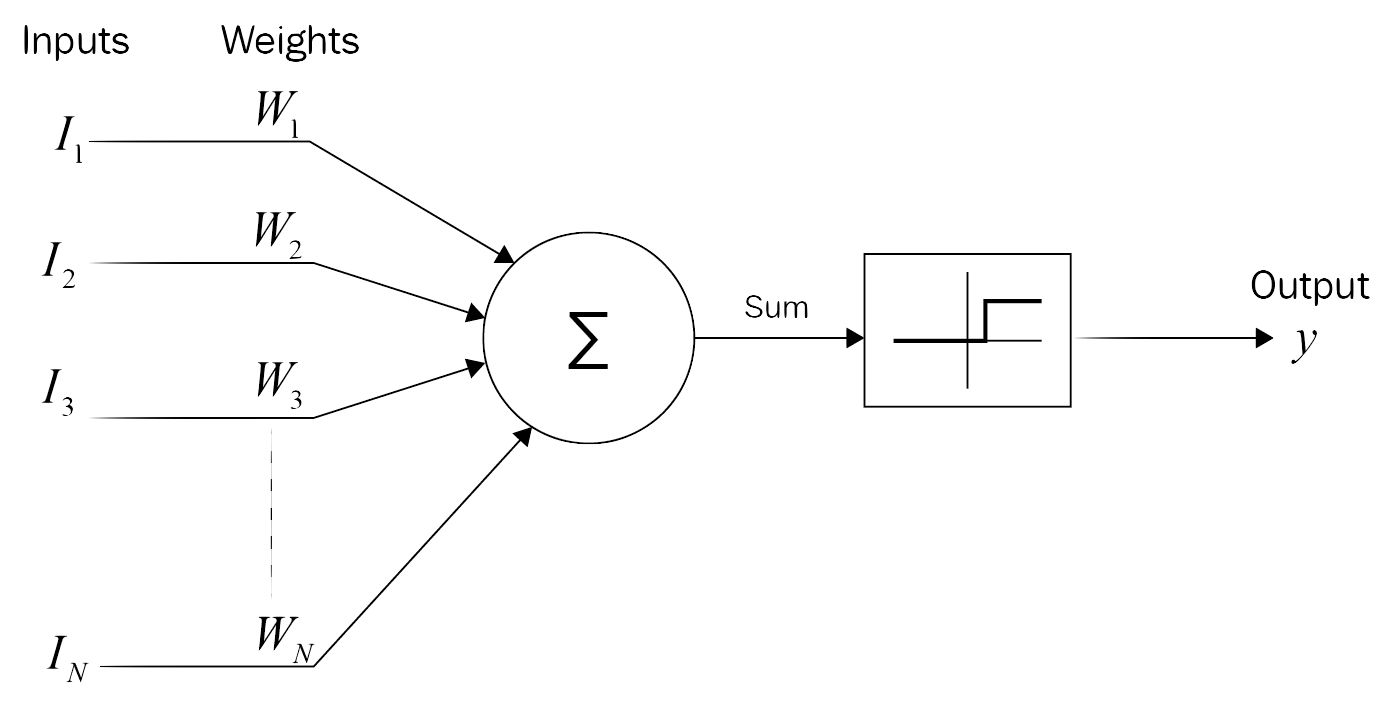
\includegraphics[scale=.25]{McCulloch-Pitts.jpg}}
\end{figure}
Consiste en unas entradas que tienen asignado manualmente un peso cada una de las que se hace el sumatorio de la entrada por el peso, este resultado se pasa por una función de activación no lineal y se obtiene la salida.
$$y=f\left(\sum_{i=1}^n I_i w_i\right) \quad f (x) = \begin{cases}1 & \textit{si}\quad  x> 0\\0 & \textit{en caso contrario}\end{cases}$$
En este momento hablamos de células individuales, no de redes.

\subsubsection{Limitaciones}
Se puede simular cualquier puerta lógica. Uniendo las puertas lógicas, se puede representar cualquier función.

El problema es el diseño de la red, que requiere determinar la arquitectura y los pesos. Se necesita un mecanismo para que determine los pesos automáticamente, es muy pesado hacerlo a mano.

El perceptrón son un conjunto de células de McCulloch-Pitts, con una sola capa, y cuyos pesos pueden ser determinados a partir de los ejemplos de los que se disponga.
\pagebreak

\subsection{Perceptrón}
Tiene una estructura similar a las células de McCulloch-Pitts, pero además de los pesos hay un umbral.
\begin{figure}[H]
	\ffigbox[\FBwidth]
	{\caption{Estructura del Perceptrón}}
	{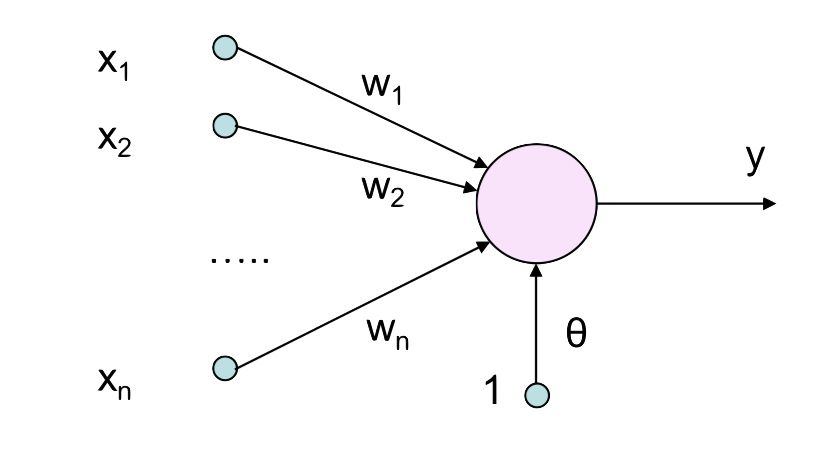
\includegraphics[scale=.35]{perceptron.jpg}}
\end{figure}

La salida de cada célula se calcula mediante:
$$y=\mathcal{F}\left(\sum_{i=1}^n x_i w_i+\theta\right) \quad \mathcal{F}(s) = \begin{cases}1 & \textit{si}\quad  x> 0\\-1 & \textit{en caso contrario}\end{cases}$$

La función escalón lo hace discriminante, si solo hay una célula y da 1 pertenece a la categoría A y si es -1 a la categoría B.

El número de células de un Perceptrón se corresponde con la dimensión de la entrada, y el número de células de salida, con el número de clases a discriminar.

En el caso binario, dos entradas una salida, el perceptrón representa una recta que divide el plano en dos partes cada una categoría.

\subsubsection{Aprendizaje}
El proceso de aprendizaje del perceptrón consiste en descubrir los parámetros de una recta que deje a todos los ejemplos de la clase A en un lado, y a los de la clase B en el otro.

Dado un conjunto de ejemplos de prueba distribuidos de los que se conoce su categoría, se trata de obtener la ecuación del hiperplano que deja a un lado los ejemplos de un tipo, y a otro los del otro.
$$A=(\vec{a}_1, ..., \vec{a}_n) \quad B=(\vec{b}_1, ..., \vec{b}_n)$$
$$\forall \vec{a} \in A,, w_1a_1+\cdot+w_na_n+\theta > 0$$
$$\forall \vec{b} \in B,, w_1b_1+\cdot+w_nb_n+\theta < 0$$
Para todos los puntos de A deben dar la misma categoría y los de B deben dar la otra.
\pagebreak

El proceso de aprendizaje necesita de un conjunto de ejemplos $\chi$ para los cuales tenemos una respuesta d($\chi$), y es un aprendizaje por refuerzo:
\begin{itemize}
	\item Si la red da una respuesta correcta, no se modifican los pesos.
	\item Si da una respuesta incorrecta, se modifican los pesos una cantidad fija.
\end{itemize}

El incremento de los pesos se realiza mediante la expresión: $\Delta w_i = d(\vec{x})x_i, , x \in \chi$

Si la \textbf{salida obtenida es y($\vec{x}$) = 1, y la deseada es d($\vec{x}$) = -1, entonces $w_i = -x_i$}. La salida es mayor que la esperada, y los pesos se decrementan

Si la \textbf{salida obtenida es -1, y la deseada es 1, entonces $w_i = x_i$.} La salida es menor que la esperada, y los pesos se incrementan.

\subsubsection{Validación}
Se realiza de forma iterativa.

\begin{enumerate}
	\item Inicialización aleatoria de los pesos y el umbral de la red.
	\item Se toma un ejemplo entrada-salida $\vec{x} = (x_1, x_2, ..., x_n), d(\vec{x})$
	\item Se calcula la salida de la red: $y(\vec{x}) = f (x_1w_1 + x_2w_2 + ... + x_nw_n + \theta)$
	\item Si $y(\vec{x}) \neq d(\vec{x})$ (clasificación incorrecta) se modifican los pesos y el umbral:
	      
	      Si $\vec{x} \in A, d(x) = 1 \rightarrow w_i(t+1) = w_i(t)+x_i, \theta(t+1) = \theta(t)+1$
	      
	      Si $\vec{x} \in B, d(x) = -1 \rightarrow w_i(t+1) = w_i(t)-x_i, \theta(t+1) = \theta(t)-1$
	      
	\item Se vuelve al paso 2 hasta completar el conjunto de patrones de entrenamiento.
	\item Se repiten los pasos 2, 3, 4 y 5 hasta alcanzar el criterio de parada.
\end{enumerate}

Cada una de las capas representa una recta por eso en el problema XOR hacían falta más capas.

\subsubsection{Tasa de aprendizaje}
Es el ritmo con el que aprende, es un valor entre 0 y 1 que regula la variación de los pesos en cada iteración, para que no se vayan mucho y oscilen.

$$w_i(t+1)=w_i(t)+\gamma d(\chi)x_i$$

Se suelen empezar con valores mayores y se va reduciendo una vez se va aproximando (balance exploración-explotación)

\section{ADALINE}
El Perceptron es de naturaleza binaria, lo que restringe su dominio de aplicación a la clasificación, pero en muchos casos se dispone de datos en el dominio de los reales. El perceptron es para clasificación lineal y ADALINE para regresión lineal.

En este caso no hay que extrapolar a qué clase pertenecen las entradas desconocidas, sino que habrá que asignar a cada entrada su valor real correspondiente.

Se trata de aproximar una función F de forma que:
$$P=\{(\vec{x}_1, y_1), ...,(\vec{x}_m, y_m)\} \quad F(\vec{x}_1)=y_1, \forall p \in P$$

No se puede utilizar aprendizaje por refuerzo, \textbf{no hay salidas correctas o incorrectas, todas son incorrectas, algunas más que otras}

En 1960, Widrow y Hoff propusieron un modelo que sí tiene en cuenta el error producido, ADAptive LInear NEuron (ADALINE)

Estructura identica al Perceptron.

La diferencia con el perceptron es la manera de utilizar la salida en la regla de aprendizaje, en el \textbf{perceptron se utiliza la salida de la funcion umbral (binaria)} para el aprendizaje (si se ha equivocado o no) y en \textbf{Adaline se utiliza directamente la salida de la red (real)} teniendo en cuenta cuánto se ha equivocado.

Se utiliza la diferencia entre el valor real esperado y la salida producida de la red $(d^p-y^p)$.

\subsection{Regla Delta}
Se define el error cometido por un modelo (un conjunto de pesos) mediante la desviación entre las salidas producidas por el mismo y las que debería haber producido, para todos los ejemplos de entrenamiento:

$$E=\frac 1 2 \sum_{p=1}^m(d^p-y^p)^2$$

El objetivo es encontrar un conjunto de pesos que haga que ese error sea el menor posible. Se aplica un proceso iterativo en el que después de propagar cada entrada, se modifican los pesos de acuerdo con la regla delta:
$$\Delta_pw_i=\gamma(d^p-y^p)x_i$$

El error es una función de los pesos por lo que tiene que haber un valor de los pesos para los que dicho error sea mínimo y para localizarlo se utiliza el método de descenso de gradiente.

El descenso de gradiente consiste en calcular la derivada de la función error respecto de los pesos en el punto determinado por el valor actual del peso, y utilizar dicho valor para variar los pesos
\begin{itemize}
	\item Si el valor es grande, es que la pendiente es grande y podemos desplazarnos mucho.
	\item Si el valor es pequeño, nos acercamos al mínimo, y variamos poco los pesos.
	\item Si el valor es cero, estamos en el mínimo y no se varían los pesos.
\end{itemize}

$$\Delta_pw_i=-\gamma\frac{\partial E^p}{\partial w_i}$$

Utilizando la regla de la cadena:
$$\frac{\partial E^p}{\partial w_i}=\frac{\partial E^p}{\partial y^p}\frac{\partial y^p}{\partial w_i}=\frac{\partial (\frac 1 2 (d^p-y^p)^2)}{\partial y^p}\frac{\partial(w_ix_i)}{\partial w_i}=-(d^p-y^p)x_i$$
De esta manera obtenemos la Regla Delta:
$$\Delta_pw_i=\gamma(d^p-y^p)x_i$$

Si aplicamos Adaline a problemas en los que las salidas son binarias la Reglas Delta quedaría:
$$\Delta_pw_i=\{ \gamma x_i \quad si \quad d^p > y^p$$

La Regla Delta es una extensión de la regla del Perceptrón para valores de salida reales.

\subsection{Procedimiento}
\begin{enumerate}
	\item Inicializar los pesos y umbral de forma aleatoria.
	\item Presentar un patrón de entrada.
	\item Calcular la salida, compararla con la deseada y obtener la diferencia: $(d^p-y^p)$
	\item Para todos los pesos y para el umbral, calcular:
	      
	      $\Delta_pw_i=\gamma(d^p-y^p)x_i,, \Delta_p\theta=\gamma(d^p-y^p)$
	\item Modificar los pesos y el umbral del siguiente modo:
	      
	      $w_j(t+1)=w_j(t)+\Delta_pw_j,, \theta(t+1)=\theta(t)+\Delta_p\theta$
	\item Repetir los pasos 2, 3, 4 y 5 para todos los patrones de entrenamiento (1 ciclo).
	\item Repetir los pasos 2,3,4,5 y 6 tantos ciclos hasta cumplir el criterio de parada.
\end{enumerate}

\chapter{Tema 2: Perceptrón multicapa}
\section{Problema XOR}
Mediante ADALINE o un Perceptrón que son aproximadores de un solo plano no es posible crear una red que represente la lógica de la puerta XOR.
\begin{table}[H]
	\centering
	\caption{Puerta XOR}
	\begin{tabular}{cc|c}
		\multicolumn{2}{l}{XOR} & \multicolumn{1}{l}{} \\ \hline
		-1 & -1 & 1  \\
		-1 & 1  & -1 \\
		1  & -1 & -1 \\
		1  & 1  & 1
	\end{tabular}
\end{table}

Se llega a un punto al aplicar estos métodos que no sabe mejorar más la solución, se estabilizan los pesos, pero es una solución muy alejada de la óptima.

Como se ha dicho solo se pueden resolver problemas en los que las salidas dependen linealmente de las entradas.

La manera de resolver este problema fácilmente es introducir una capa adicional, que es como emplear dos rectas para discriminar.

En el caso de más de 1 capa para ajustar los pesos no podemos hacerlo como anteriormente, ya que en las capas ocultas no conocemos la salida, solo nos serviría para la capa de salida.

\section{No linealidad}
En la mayoría de los casos los datos se distribuyen de manera no lineal, por lo que en general las rectas no son útiles para solucionar los problemas reales. Se necesitan curvas complejas.

\section{Función de activación}
Es necesario incluir una función de activación no lineal en la salida de las células. 

Es importante que sean no lineales, derivables y acotadas.
\pagebreak

Nosotros emplearemos:
\begin{itemize}
	\item Función Sigmoide (0 - 1)
	      $$g(x)=\frac{1}{1-e^{-x}}\quad g'(x)=g(x)(1+g(x))$$
	\item Tangente Hiperbólica (-1 - 1) $$g(x)=\frac{e^x-e^{-x}}{e^x+e^{-x}} \quad g'(x)=1-g(x)^2$$
	\item Unidad de Rectificado Lineal - ReLU $$g(x)=\max(0,x) \quad g'(x)= \begin{cases}1 & x > 0\\0 & \textit{en otro caso}\end{cases}$$
\end{itemize}

\section{Redes alimentadas hacia delante}
En cada capa C se calcula la salida de las células que la componen $a^C_j$ con: 
$$y^C_j=f\left(\sum^{C-1}_{i=1} w^{C-1}_{ij}y^{C-1}_i+\theta_j^C\right)=f(s^{C}_{j})$$

Tal que $w^C_{ij}$ es el peso de la capa C entre la célula origen i y la célula destino j y $y^{C-1}_j$ es la salida de la célula i de la capa anterior. El sumatorio se hace para todas las células de la capa anterior.

\section{Aprendizaje de pesos}
En este caso no podemos hacer como en ADALINE, ya que solo se conoce la salida esperada para la última capa, pero para las intermedias no podemos. Solo podríamos ajustar los pesos de esta. 

Es por esto por lo que en 1986 Rumelhart et al. presentaron una generalización de la Regla Delta que solucionaba este problema: \textbf{Regla Delta Generalizada}.

\section{Función de error}
El objetivo es que la red produzca resultados los más parecidos a los deseados, depende del tipo de problema.
\pagebreak

En los problemas de \textbf{Clasificación} se utiliza la \textbf{entropía cruzada}: $E=-\sum^C_{i=1}d_i \log (y_i)$ La base del logaritmo depende del número de posibles valores.
\begin{itemize}
	\item No siempre es conveniente ahorrar bits cuando se hace clasificación, ya que el conocimiento depende de las conexiones.
\end{itemize}

En \textbf{Regresión} se utiliza el \textbf{error cuadrático medio}: $E=\frac 1 N \sum^N_{i=1} (d_i-y_i)^2$

Se puede hacer una representación gráfica del error según los pesos que nos permite ver como se distribuyen y buscar los valles, pero esto no es posible de dibujar en los problemas por el gran tamaño de los espacios y coste. Lo que se hace es como no conocemos el error en todos los puntos se utiliza la derivada para ver la pendiente y reducirla en busca de un mínimo local (Problema del mínimo local, es difícil salir).

Como el objetivo es minimizar la función de error se calcula el gradiente de la función en un punto W para ver la pendiente y como queremos minimizar iremos en dirección opuesta al gradiente hasta alcanzar convergencia.

\section{Retropropagación del gradiente}
Hay que calcular la derivada del error respecto a cada uno de los pesos, dicha derivada se utilizará para modificar el peso correspondiente.

Se va aplicando la regla de la cadena, en las capas intermedias hay que calcular los valores hacia atrás.

La idea es desplazar el vector de pesos siguiendo la dirección negativa del gradiente del error en dicho punto, de esta manera nos aproximamos al mínimo error.
\section{Procedimiento BackPropagation}
\begin{enumerate}
	\item Se inicializan los pesos y umbrales de la red (valores aleatorios próximos a 0)
	\item Se presenta un patrón n de entrenamiento, $(x(n),s(n))$, y se propaga hacia la salida, obteniéndose la respuesta de la red $y(n)$
	\item Se evalúa el error, $e(n)$, cometido por la red para el patrón n
	\item Se aplica la regla delta generalizada para modificar los pesos y umbrales de la red:
	\begin{enumerate}
		\item Se calculan los valores $\delta$ para todas las neuronas de la capa de salida
		\item Se calculan los valores $\delta$ para el resto de las neuronas de la red, empezando desde la última capa oculta y retropropagando dichos valores hacia la capa de entrada
		\item Se modifican pesos y umbrales
	\end{enumerate}
	\item Se repiten los pasos 2, 3 y 4 para todos los patrones de entrenamiento, completando así un ciclo de aprendizaje
	\item Se evalúa el error total cometido por la red (error de entrenamiento)
	\item Se presentan los patrones de validación, calculando únicamente la salida de la red (no se modifican los pesos) y se evalúa el error total en el conjunto de validación
	\item Se repiten los pasos 2, 3, 4, 5, 6 y 7 hasta que:
	\begin{enumerate}
		\item El error de entrenamiento permanece estable
		\item El error de validación permanece estable
		\item El error de validación empieza a aumentar
	\end{enumerate}
\end{enumerate}

\section{Retropropagación del gradiente}

$$s^P_k= \sum_j w^{P-1}_{jk}y^{P-1}_j+\theta_k^P \quad y^P_k=f(s^P_k)$$

Necesitamos para cada célula un valor delta (menos para la entrada). Se deriva en función de la entrada, ya que es lo que cambia el error. $\delta$ Estimación del error en esa célula.

$$\delta^P_k=-\frac{\partial E}{\partial s^P_k}=-\frac{\partial E}{\partial y^P_k}\frac{\partial y^P_k}{\partial s^P_k}=-\frac{\partial E}{\partial y^P_k}f'(s^P_k)$$

\textbf{Para la salida (o):} Siendo el error $E=\frac 1 2 \sum (d^o_k-y^o_k)^2$
$$\delta^o_k=-\frac{\partial E}{\partial y^o_k}f'(s^o_k)=-[-(d^o_k-y^o_k)]f'(s^P_k)=(d^o_k-y^o_k)f'(s^o_k)$$

\textbf{Para la oculta (h):} Tras calcular la capa de salida, va hacia atrás estimando la salida deseada de las capas ocultas.
$$\delta^h_k=-f'(s^h_k)\frac{\partial E}{\partial y^h_k}=-f'(s^h_k)\sum^{m}_{l=1}\frac{\partial E}{\partial s^{h+1}_l}\frac{\partial s^{h+1}_l}{\partial y^h_k}=-f'(s^h_k)\sum^{m}_{l=1}[-\delta^{h+1}_l]\frac{\partial (\sum_j^n w_{jl}y^{h-1}_j)}{\partial y^h_k}=$$ $$=f'(s^h_k)\sum^{m}_{l=1}\delta^{h+1}_l w_{kl}$$
\pagebreak

\section{Retropropagación del error}
Se calcula un valor, llamado $\delta$, para todas las células de la red, empezando por las de la última capa y retrocediendo una capa en cada iteración.

El valor delta es proporcional a la derivada del error estimado por la célula.
\begin{itemize}
	\item En la última capa se conoce el error producido por las células, y el delta se calcula teniendo en cuenta ese error.
	\item En las capas ocultas, se propaga hacia atrás el valor $\delta$ ponderado por los pesos.
\end{itemize}

Una vez calculados los deltas, todas las conexiones se actualizarán de la misma manera: 
\begin{figure}[H]
	\ffigbox[\FBwidth]
	{\caption{Retropropagación del error}}
	{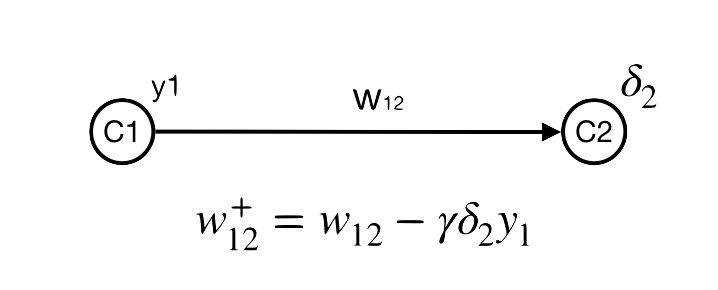
\includegraphics[scale=.35]{regla-delta.jpg}}
\end{figure}
$$w^+_{ij} = w_{ij}-\gamma \delta_j y_i \quad b^+_{i}=b_i - \gamma \delta_j$$

\section{Tasa de aprendizaje $\gamma$}
Valor empleado en la regla delta por el que se multiplica la $\Delta w_i$. 

Cuanto más grande más rápido nos aceptamos a la solución, pero cuidado porque si es muy alto oscilaremos y no nos acercaremos. 

Si es muy pequeño la convergencia será muy lenta y puede ser inviable al ralentizar el proceso, estancándose en mínimos locales.

Encontrar la tasa de aprendizaje óptima no es trivial, se trata de asignar el mayor valor posible  sí que se produzca oscilación.

Una manera de evitar la oscilación es hacer que el cambio de los pesos dependa de  la intensidad del cambio anterior, velocidad con la que varía, una especie de inercia llamada momento. Evita que puedan diferir en exceso.
\pagebreak

\section{Momento}
Término que recoge el cambio producido por los pesos en la iteración precedente:
$$m(t) = w(t) - w(t - 1) = \Delta w(t)$$
$$w_{jk}(t + 1) = w_{jk}(t) + \gamma \delta^p_k y^p_j + \alpha\Delta w_{jk}(t)$$
$\alpha$ es la intensidad que le queremos dar a la inercia.

Contrarresta las oscilaciones restando cuando cambia de sentido, se pueden utilizar tasas de aprendizaje relativamente altas, lo que permite una convergencia rápida. Permite navegar más eficazmente por la función de error.

\section{Generalización}
La red adapta sus pesos a partir de los ejemplos de entrenamiento hasta formar un modelo final, esta capacidad permite comportarse correctamente más allá de estos. Aunque existe un riesgo de que solo conociendo los de entrenamiento no sepa generalizar.

El conjunto de ejemplos sea suficientemente grande y característico.

El modelo resultante debe ser válido para cualquier situación, no solo para los datos de entrenamiento.

\section{Sobre-aprendizaje}
El módulo se ajusta a los datos de entrenamiento de una manera demasiado precisa. Dejando de generalizar, cosa no deseable.

Si se entrena poco, la aproximación que genera el modelo es muy burda.

Si se entrena mucho, puede adaptarse solo a los ejemplos de entrenamiento, como si lo memorizara.

Cuando el error de validación deja de disminuir, la red empieza a sobreentrenar, y debe pararse el entrenamiento

No solo depende de los ciclos de aprendizaje, también de:
\begin{itemize}
	\item Excesivo número de pesos o neuronas ocultas, se ajusta con mucha exactitud.
	\item Excesiva complejidad del modelo en relación con el número de patrones de entrenamiento. Hacer las redes más sencillas.
	\item Escasez de patrones de entrenamiento, por lo que se adapta rápido a estos patrones y pierde la capacidad de generalización.
\end{itemize}

\section{Conjunto de validación}
Conjunto de datos diferentes a los de entrenamiento para comprobar la capacidad de generalización del modelo, no se utiliza para entrenar, solo para verificar la generalización y decidir cuándo parar. El conjunto de entrenamiento se divide en dos, uno para entrenar y otro para validar.

Se utiliza para saber cuándo empieza a sobreentrenar.

Los datos de validación deben tener una estructura similar a los de entrenamiento, para esto se aleatorizan los datos y hacer que sean menos sesgados posibles.

Si hay correlaciones entre entrenamiento y validación, las dos curvas se comportaran parecido y nos servirá para ver la generalización.

\section{Regularización}
A veces se necesitan muchas neuronas para determinados problemas y para evitar sobreajuste lo que se hace es eliminar de manera aleatoria un porcentaje de las neuronas (10-25 \%) en cada iteración, así no puede sobreaprenderlo.

Esto reduce la capacidad de memorizar, haciendo que tenga que aprender patrones y no casos concretos.

Se ha probado experimentalmente la eficacia de redes en las que las señales solo recorren parte de la red.

\section{Actualización por lotes}
La actualización de los pesos se puede realizar:
\begin{itemize}
	\item Después de introducir un dato. $E= \frac{1}{2} (y-x)^2$
	\item Después de introducir todos o una serie de datos. $E= \frac{1}{N} \sum_{i=1}^N(y_i-x_i)^2$
\end{itemize}
Lo recomendado es tras una serie de datos, ya que tras cada patrón es muy costoso computacionalmente o si lo hacemos tras todo el conjunto de entrenamiento dificulta que la red pueda generalizar bien.

Hacer estas series de datos muy grandes hace que sea muy rápido computacionalmente y si son muy pequeños mejora la generalización.

Hacerlo por lotes permite una mejor estimación del gradiente, produce una convergencia más suave y utilizar tasas de aprendizaje más grandes, por lo que aprende más rápido.

Es paralelizable, lo que permite incrementar más aún la velocidad del aprendizaje.

\section{Validación cruzada}
Es un método para la evaluación de modelo que lo que permite es entrenar la red con diferentes valores de parámetros para quedarnos con el mejor. 

Aunque que se obtenga mejor evaluación no implica que se comporte mejor ante ejemplos desconocidos, por esto que para generar modelos es necesario un conjunto de ejemplos que no hayan sido utilizados en el entrenamiento, ni para modificar los pesos y tampoco para establecer el criterio de parada. 

Los modelos deben ejecutarse el suficiente número de veces con diferentes inicializaciones y asignar la media de los resultados.

Un modelo es mejor que otro si la media de los errores de test es estadísticamente significativa menor en una que en otro.

Se divide el conjunto de entrenamiento en x particiones, para hacer x modelos (x+1 en total) que se entrenaran con todas las particiones menos 1 y se hará test con la otra restante.

Para cada modelo se hace una serie de veces para evitar el sesgo del inicio aleatorio. Cuando se ha completado se hace la media del error y ese será el error del modelo que se genera si se entrena con el conjunto completo de datos y esos parámetros.

En todos los modelos una parte será para validación.

\section{Debilidades}
\subsection{Mínimos locales}
Si existen valores de la función de error con valores bajos rodeados extensamente por valores más altos, la red puede quedarse estancada y no acceder a valores mejores del error.

Soluciones:
\begin{itemize}
	\item Añadir ruido al método de descenso del gradiente
	\item Partir de diferentes inicializaciones aleatorias
	\item Aumentar el número de neuronas ocultas
\end{itemize}

\subsection{Saturación}
Cuando la entrada total de una célula toma valores muy altos, la salida permanece constante por saturación, debido a la naturaleza de la función de activación.

El problema está en la función de activación.

Si la entrada sigue aumentando, esto no produce variaciones en la salida

La modificación de los pesos en una célula depende de la salida: $y_k(1 - y_k)$

Si la salida está cercana a 1, lo cual ocurre en la zona de saturación, los pesos dejan de modificarse y se produce estancamiento.

Soluciones:
\begin{itemize}
	\item Normalizar datos de entrada
	\item Comenzar con valores de pesos cercanos a cero
	\item Utilizar otras funciones de activación: ReLU
	
	Impide la saturación de las salidas a un valor de 1 que detiene el aprendizaje
	
	Permite generar muchos valores cero como salida de neuronas, lo cual las desactiva y asemeja más a modelos biológicos.
\end{itemize}

\chapter{Tema 3: Modelos de Redes de neuronas no supervisados}
Tenemos un conjunto de datos y ya, sin clases o etiquetas, queremos saber que se puede decir de ellos.

La tarea más habitual es el agrupamiento o clustering en función de características comunes de los datos.
\section{No supervisado}
La red descubre por sí sola características, regularidades, correlaciones, categorías, …, de los datos de entrada, a esto se le llama auto-organización. 

Solo es relevante si los datos muestran algún tipo de redundancia $\nRightarrow$ aleatoriedad. Si tienen algún tipo de estructura.

Tareas principales:
\begin{itemize}
	\item \textbf{Análisis de componentes principales:} Determinar qué entradas caracterizan principalmente a los datos. Si se eliminan, los datos tendrían una estructura similar.
	\item \textbf{Agrupamiento:} Dividir el espacio de entrada en regiones.
	\item \textbf{Prototipado:} Definir las regiones mediante prototipos.
	\item \textbf{Codificación:} La salida es una versión reducida de la entrada.
	\item \textbf{Extracción de características:} La red produce respuestas similares ante entradas similares.
\end{itemize}

\section{Modelo biológico}
Alta dimensionalidad $10^{11}$-$10^{14}$ células, con 1000-10000 conexiones cada una y una velocidad de 1 ms.

Aprendizaje continuo. No hay fase de aprendizaje y fase de funcionamiento. Se aprende en todo momento.

Focalización en estímulos relevantes. Aprendizaje por repetición de estímulos. Plasticidad.

\subsection{Reglas de Hebb}
Cuando el axón de una célula A está lo suficientemente cerca como para excitar a una célula B y repetidamente toma parte en la activación, ocurren procesos de crecimiento o cambios metabólicos en una o ambas células de manera que tanto la eficiencia de la célula A, como la capacidad de excitación de la célula B se ven aumentadas.

En la regla de Hebb la modificación de los pesos no obedece a ningún factor externo.

La conexión entre dos células se verá aumentada si ocurre que las dos se encuentran activas a la vez de manera persistente. Aquellas que no se repiten con frecuencias, se irán debilitando y se acabarán olvidando.

$$\Delta w_{ij}=a_i\cdot a_j \quad\quad\quad\quad \Delta w_{ij}=\mu(a_i - \overline{a_i})\cdot(a_J- \overline{a_j})$$
$$\Delta w_{ij}=\Delta a_i\cdot \delta a_j \quad\quad\quad\quad \Delta w_{ij}= \mu a_i w_{ij} \Delta a_j$$
$$\frac{dw_{ij}}{t}=-w_{ij}+a_i\cdot a_j \quad\quad\quad\quad \frac{dw_{ij}}{t}=-w_{ij} + \sigma(a_i) \cdot \sigma(a_j)$$

Este tipo de aprendizaje se utiliza de forma generalizada en casi todos los modelos no supervisados, es la regla que se utiliza de manera normal en este tipo de procesos.

\section{Modelo de Interacción lateral}
Una de las características del cerebro es que está estructurado, este modelo trata de emular este tipo de conexiones estructuradas, de manera que hay partes que están más especializadas en una determinada tarea.

Estudios sobre el neocórtex muestran una estructura bidimensional por capas conectadas mediante conexiones laterales.

Cada célula se conecta a las más cercanas mediante conexiones excitatorias y a las más lejanas con inhibitorias. Las conexiones (-) (+) pierden intensidad con la distancia entre células. Al propagarse las señales mediante este esquema, se producen zonas más activadas y menos.

Un modelo artificial de célula (c) podría ser: $y_c^{t+1}=\sum^n_{i=1} x_i w_{ic} - \sum^n_{k=1} y_k w_{kc}+y^T_C w_{cc}$.


Primer parte las entradas normales, $w_{kc}$ células colindantes, $w_{cc}$ conexiones recurrentes excitatorias con si mismo. La y será $y_i = f \left(\sum^l_{j=-l} w_{ij}y_j\right)$

Donde los pesos w$_{ij}$ tendrían valores siguiendo la función $f(x) = (1 - x^2)e^{- \frac{x^2}{2}}$, la función sombrero mejicano.

El eje horizontal (x) representa la distancia entre las células, el vertical (y) el valor del peso.

Si la distancia es corta, el peso es positivo y grande.

Disminuye con la distancia hasta hacerse negativo, para acabar siendo cero.

No es un modelo de red neuronal, porque no tiene aprendizaje, pero es utilizado, por su característica espacial embebida en otros modelos neuronales.

\section{Aprendizaje competitivo - CL}
Se trata de asignar, a una misma categoría, aquellos datos de entrada que compartan ciertas características.

Compuesto por dos capas, una de entrada, y una de salida con tantas células como categorías (capa competitiva) y cada célula de la capa competitiva se corresponde a una categoría.

Cuando llega un dato, lo deseable es que se active, en la capa competitiva, solo aquella célula que corresponda con la categoría a la que pertenece dicha entrada. Los datos de entrada no están etiquetados. La red debe asignar la misma categoría a datos similares.

En la capa competitiva:
\begin{itemize}
	\item Todas las células están conectadas con las demás.
	\item Los valores de los pesos son fijos y siguen el esquema de interacción lateral.
	\item Las conexiones de las células consigo mismas toman valores positivos, iguales para todas ellas.
	\item Las conexiones con las demás células toman valores negativos, los mismos para todas.
\end{itemize}

Entre la capa de entrada y la competitiva.
\begin{itemize}
	\item Las conexiones son excitatorias.
	\item Varían a medida que avanza el aprendizaje.
\end{itemize}

\subsection{Funcionamiento}
F1 es la capa de entrada y F2 es la competitiva o salida.
\begin{enumerate}
	\item Las entradas se propagan de F1 a F2.
	\item A cada célula de F2 llega la misma entrada, pero ponderada por sus conexiones que son diferentes.
	\item Cuando la señal llega a F2, se desactivan las conexiones F1 $\rightarrow$ F2.
	\item La señal es propagada de forma síncrona por F2.
	\item F2 se estabiliza cuando todas las células producen salida cero, excepto una.
	\item La célula que reciba más señal al principio, se queda con toda la señal y es la célula ganadora.
	\item Se asignará a la entrada la categoría relacionada con la célula ganadora.
	\item Cuando se introduce un nuevo dato, se restablecen las conexiones F1 $\rightarrow$ F2.
\end{enumerate}

Lo ideal es que se vaya inhibiendo unas a otras de tal manera que todas excepto 1 queden muy cercanas al 0, la que toma el 1 es la que aprenderá.

\subsection{Aprendizaje}
En F2 (salida) no hay aprendizaje, los pesos entre sus células son fijos: $\forall i \quad \sum^N_j w_{ij}=1$ y $\forall i, j \quad w_{ij}=w_{ji}$.

Los valores que van de una célula a otra en F2 tienen el mismo que la conexión contraria. Además los pesos se normalizan, de manera que todas en un sentido sumen 1.

Entre F1 y F2 aprende “el que gana se lleva todo”: Para las células no ganadoras será 0, para las ganadoras será $\frac{dw_{ij}}{dt}=[-w_{ij}+\theta_i]$. $\theta_i=\frac{I_i}{\sum_{j=1}^M I_j}$

\subsection{Características y limitaciones}
Se trata de un aprendizaje Hebbiano. El aprendizaje es proporcional a las salidas producidas por las células que une.

Se refuerzan más las conexiones por las que pasa más señal (las que tienen un mayor I$_i$).

No produce codificación estable ante entradas arbitrarias. La introducción de entradas aleatorias o con ruido, produce salidas arbitrarias, y puede afectar a lo ya aprendido.

Capacidad limitada de codificación (con muchas entradas y pocas categorías se puede colapsar y dejar de aprender).

Se necesita establecer a priori el número de categorías. Lo normal es tener un número intuitivo de salida e ir probando, se evaluará con la dispersión de clústeres, se busca tener pocos clústeres y bajo dispersión.

\section{Mapas auto-organizativos de Kohonen - KSOM}
El modelo de aprendizaje competitivo se puede extender para realizar tareas de agrupamiento no supervisado.

En ese caso cada célula de la CC se corresponde con el centroide de un agrupamiento.

Un punto del espacio de entrada pertenece al agrupamiento representado por el centroide más cercano a él.

De esta manera se divide el espacio en regiones de Voronoi.

\subsection{Modelo}
Cada célula de la capa competitiva (CC) está conectada con todas las entradas. Si la entrada tiene dimensión “n”, cada célula de la CC tendrá “n” conexiones.

Se puede representar cada célula de la CC como un punto en un espacio n-dimensional.

La señal se propaga desde la entrada de manera no habitual.

Para cada célula de la CC, se calcula la distancia entre sus pesos, y los valores de la entrada. Se calcula la distancia desde cada entrada hasta cada prototipo.

La activación de la célula coincide con dicho valor de distancia.

Se puede elegir entre varias medidas de distancia:
\begin{itemize}
	\item Producto escalar: $\tau_j=d(e,w_j)=\sum_i e_iw_{ij}$. e es la entrada, w es el peso de la entrada-célula, y $d(x, y)$ es la distancia.
	\item La más utilizada es la euclídea: $\tau_j= \sqrt{\sum_i (e_i - w_{ij})^2}$.
\end{itemize}

\subsection{Funcionamiento}
\begin{enumerate}
	\item Se recibe el vector de entrada y se propaga por las conexiones hasta llegar a la capa de competición mediante alguna de las fórmulas anteriores.
	\item Cada neurona de la CC produce una salida al comparar la entrada con sus pesos, la competición sigue el modelo de interacción lateral. Calcula las distancias.
	\item Se selecciona aquella que produzca una salida más pequeña (célula ganadora, la más cercana).
\end{enumerate}

Cuando ya tienes las distancias de CC y entrada se cortan las conexiones con la entrada y se deja funcionar la interacción lateral hasta que quede un 1 y el resto 0. Aunque lo normal es coger la que tiene menor distancia y no hacer interacción lateral.

\subsection{Aprendizaje}
El aprendizaje se produce en los pesos entre la entrada y la competición, siguiendo un esquema Hebbiano.

Emplea la regla “el que gana se lleva todo”: 0 para las no ganadoras y para la ganadora $\frac{dw_{ij}}{dt}=\alpha(t)\tau_j (e_i(t)-w_{ij}(t))$.

La tasa de aprendizaje varía en función del tiempo, va decrementando con el tiempo una cantidad constante. Se utiliza para que los valores más antiguos tengan mayor intensidad de aprendizaje. $\alpha(t+1)=\alpha (t) - \beta$.

Mediante el valor de $\beta$ se determina el número de ciclos tota les de aprendizaje, $\textit{Iteraciones}=\frac{\alpha(0)}{\beta}$, que serán las veces que se puede decrementar el valor hasta llegar a 0.

Los pasos son:
\begin{enumerate}
	\item Se introduce un patrón de entrenamiento.
	\item Se calcula su distancia a todos los prototipos de la CC.
	\item Se selecciona el de menor distancia C$_j$ (célula ganadora).
	\item Las conexiones de las células ganadoras se modifican, acercando sus coordenadas a las de la entrada: $w_{ij}=\alpha(e_i - w_ij)$.
	
\end{enumerate}

\subsection{Vecindario}
Al final del aprendizaje cada célula se situará en el centro geográfico de los patrones a los que representa.

Cada célula es independiente y no aporta información sobre las demás, por lo que sería interesante incluir información de cómo se relacionan las células entre sí (como se relacionan las categorías entre sí).

En SOM esto se puede hacer introduciendo el concepto de vecindario, cada célula tiene un conjunto de vecinos, que influirán en su aprendizaje. Se forma una rejilla que puede ser unidimensional o bidimensional.

La distancia entre dos células es el número de células por las que hay que pasar para llegar de una a otra y la distancia de una célula consigo misma es 1.

Este añadido se utiliza en el aprendizaje, cuando una célula gana, también se modificarán las vecinas según la distancia. La regla de aprendizaje pasa aento ser:

$$\frac{dw_{ij}}{dt}=\frac{\alpha(t)}{d(c_i, c_j)} (e_i(t)-w_{ij}(t))$$

De manera que $c_i$ es la ganadora y $d(c_i, c_j)<\theta$ es la distancia entre la ganadora y la vecina j, que debe estar a menos de una distancia umbral, para el resto de las células será 0.

En este caso el aprendizaje se produce en la célula ganadora y en sus vecinas, la intensidad del aprendizaje decrece con la distancia a la célula ganadora hasta que más allá de un determinado umbral $\theta$ no se produce aprendizaje.

Para cada patrón de entrenamiento se elige una célula que se desplazará en dirección a dicho patrón y en su movimiento arrastra a las que están conectadas con ella, hasta un determinado rango. Esto hace que células próximas en la topología de la red representen agrupamientos similares.

Al final, células cercanas en el vecindario ocuparán posiciones cercanas en el espacio y esto permite no solo dividir las entradas en grupos, sino relacionar los grupos entre sí.
\subsection{Procedimiento}
\begin{enumerate}
	\item Inicialización pesos a valores aleatorios pequenos.
	\item Presentar una nueva entrada. Actualizar ALPHA
	\item Progpagar la entrada hsta la capa de competición donde se seleccina una celula ganadora.
	\tem Actualizar los peso de la celula ganadora y sus vecinas.
	\item Si aun quedan entradas, ir a 2.
	\item Actualizar ALPHA
	\item Ordenar el conjunto de aprendizaje.
	\item Si ALPHA esta por encima de un cierto umbral, ir al 2.
\end{enumerate}
\subsection{Ejemplo de problema del viajante}

El metodo que se utiliza es el de Kohonnen de la goma elastica, dado que se va estirando y adaptando al dibujo de las ciudades, segun se estira se aumentan las celulas.

El veciandario aporta informaicón adicionla sobre la estructura de los agrupamientos, en este caso el vecindario es fundamental, es lo que realmente nos interasa no la ubicación de las celulas.

Se realizan las siguientes modificaciones:
	\begin{itemize}
	
	\item Se cran un vencidario unidmensional cirula en forma de anillo, como si fuera una goma elastica, tendar solo dos conexiones con otras celulas, una en el ado dereco y otra en el lado izquierdo.
	\item Se comenzara con pocas celulas, como son 3, buscando que se vayan moldenado y acercando los puntos. Tras realizar un ciclo/iteración completa, haber pasado por las entradas las ciudades que componen el problema, en este momento se dividen las celulas en otras dos.
	\item En este caso cada celula tiene varias ciudades asignadas, por esto es por lo que se particiona, dado el caso de que no tenga asignada ninguna ciudad esta celula se elimina.
\end{itemize}

El punto final es que tengamos tantas celulas como ciudades, de manera que cada una corresponda con una ciudad y las conexiones con las otras dos el camino que se debe recorrer, es decir el vecindario es la solución.

\section{K-medias}
Fue propuesto por J. MacQueen en 1967.

Algoritmo de agrupamiento no supervisado, el espacio de patrones de entrada se divide en K clusters o regiones.

Es necesario establecer el numero de clusters (K)

Dado un conjunto de patrones: $X(n)=(x_1(n), x_2(n), ...x_p(n)) n=1, ... N$ se pretende encontrar K centros $C_i =....$ con el objetivo de minizar la distancias euclideas entre los patrons de entrada y el centro mas cercano.
$$D=\sum^k_{i=1}\sum^N_{n=1} Min ||X(n) - C_i||$$

	N esl numero de patrones, || || representa la distancia euclidea, X(n) el patron de entrada n y Min es la función de pertenencia.
	
	$$Min = 1 si ||X(n) - C_i|| < || X(n) - C_s || \forall \neq i   0 en caso contrario$$

Se trata de encontrar los K puntos de la región que se genera con todas las entradas, que mejor representa a todos los datos, cada uno de los punto generará un cluster que estara compuesto por aquello puntos que se encuntrar mas cerca de ese cluster que de ningun otro.

Los punto C se generaran incialmente aleatoriamente, y segun que instancias esten mas cerca de este que de otro, se calculara la media de sus entradas de manera que se centre para todas estas, esto repetido para todos los puntos y multiples veces hace que se vayan centrando poco a poco y distribuyendo.

\subsection{Procedimiento}
\begin{enumerate}
	\item Se inicializan aleatoriamente los centros de los K clusters.
	\item Se asignan $N_i$ pattrones de entrada a cada cluster $C_i$. El patron X(n) pertenede al cluster $C_i$ si: FORMULA
	\item Se calcula la neuva posición de los centroiddes como la media de todo slo patrones que perteencen al cluster, es decir: FORMULA
	\item Se repiten los pasos 2 y 3 hasta que las nuevas posiciones de los centroides no se midifican respecto a su posició anterior.
		FORMULA
	\end{enumerate}
	
\subsection{Resumen}
...

\section{Learning Vector Quantization}
Cuando Kohonen creo su modelo vio que podia se aplicable en casos de aprendizae supervisado, como clasificación, no solo para clustering (no supervisado). Emplearlo conociendo las salidas nos permite dividir las regiones de manera mas facil.

Se combina el aprendizaje competitivo con el supervisado.

Se mantiene la tarea de dividir el espacio en regiones, pero estas regiones representaran las etiquetas de la clase de manera que dependiendo de la región en la que caiga una nueva instancia pertenecerá a la clase correspondiente.

Lo que se busca es reducir el numero de errores de clasificación cuando se introducen los patrones de entrada.

Segun las regiones de Voronoi que se generen.

Las celulas estaran etiquetadas e inicialmente se elige el numero de celualas que tendra el modelo y cuales son sus etiquetas (no solo hay una neurona por etiqueta), debe haber al menos mas del doble que el numero de etiquetas.

La unica variación el es el proceso de aprendizaje.

Las entradas son del tipo: $E_i = [(e_1^i, C),(e_2^i, C), ..., (e_n^i, C)],, i = 1...m$

\subsection{Reglas de aprendizaje}
\begin{enumerate}
	\item Se inicializan los pesos a valores pequenos aleatorios.
	\item Para cada uno de los patrones de entrada, se propada por l ared y se obtiene la celula ganadora.
	\item Si la celula ganadora pertenece a la misma categoria que la entrada.
	\item Se modifican los pesos de la celula ganadora siguiendo las ecuaciones de KSOM: $\Delta w_{ij} = \alpha (e_i - w_{ij}$
	\item Si la celula ganadora no pertenece a la misma categoria que la entrada.
	\item Se modifican los pesos de forma inversa a los de KSOM: $\Delta w_{ij} = - \alpha (e_i - w_{ij}$
	\item Repetir los pasos 2-7 hasta que se cumpla el criterio de parada.
\end{enumerate}

Si la red produce una respueta correcta, acercamos el prototipo al dato de entrada.

Si la red produce una respuesta incorrecta, alejamos el prototipo al dato de entrada.

Al final del proceso los prototipos se colocaran en el centro de masas de puntos etiquetados con su misma categoria.

\section{LVQ2}
METER DIAPOS AL IPAD

Se calculan dos celulas gandoras, las dos mas proximas.

Si las dos pertenecen a la misma clase, solo se aprende la mas cercana, siguiendo la reglas del LVQ:
	FORMULA
	FORMULA
	
Si cada una pertenece aun clase, la de la misma clase de la entrada se acerca, la otra se aleja.

Variante LVQ2.1: Solo se aprenden los dos prototipos mas cercanos si:
\begin{itemize}
	\item Pertenecen a clases diferentes.
	\item Estan dentro de una ventana ($\theta$) del plano medio de los dos vectores.
	$\min \left(\frac{d_i}{d_j}, \frac{d_j}{d_i} \right) > \frac{1-\theta}{1+\theta}$
	
	Se divide el mas grande sobre el mas pequeno.
\end{itemize}


\end{document}